\clearpage
\subsection{premi/client/editor}
\begin{figure}[H]
\begin{center}
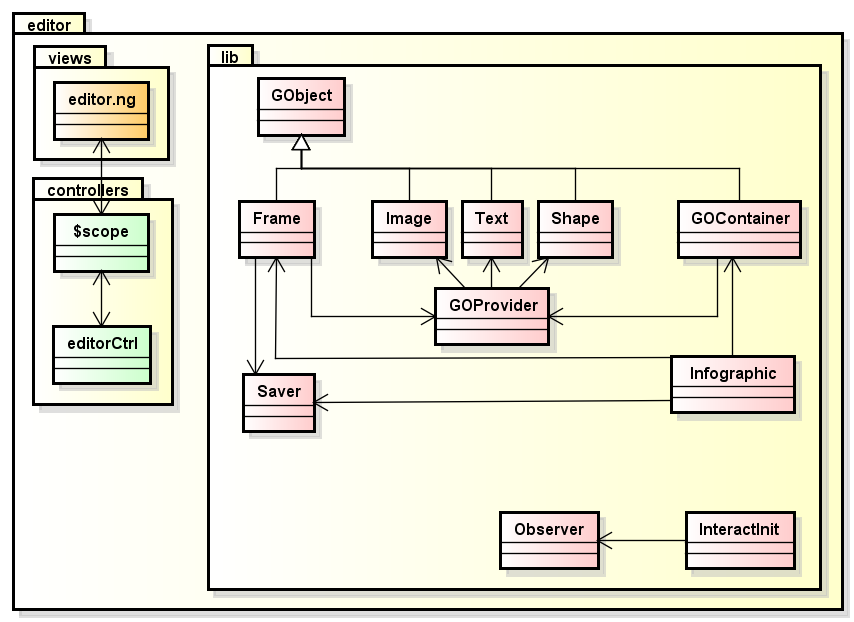
\includegraphics[scale=0.70]{img/diapkg/editor.png}
\caption{Diagramma della classe premi/client/editor}
\end{center}
\end{figure}

%-------  diagramma di un template %
\subsubsection{premi/client/editor/views/editor.ng}

\begin{description}
%-------  descrizione del template%
\item[Descrizione] \hfill
	Template della vista associata allo \textit{\$scope} di \textit{editorCtrl}. Fornisce uno scheletro per le altre viste dedicate alla gestione dell'editor. 
\end{description}

%-------  diagramma di un template %
\subsubsection{premi/client/editor/views/basicToolbar.ng}

\begin{description}
%-------  descrizione del template%
\item[Descrizione] \hfill
	Template della vista associata allo \textit{\$scope} di \textit{basicToolbar}. Fornisce il menù per:
	\begin{itemize}
	\item accedere al frameEditor;
	\item accedere all'infographicEditor;
	\item accedere al trail Editor.
	\end{itemize}
\end{description}

%-------  diagramma di un template %
\subsubsection{premi/client/editor/views/shapeMenu.ng}

\begin{description}
%-------  descrizione del template%
\item[Descrizione] \hfill
	Template della vista associata allo \textit{\$scope} di \textit{editorCtrl}. Fornisce la lista contenente gli shape disponibili che possono essere inseriti in un frame.
\end{description}


\subsubsection{premi/client/editor/controllers/editorCtrl}
\begin{figure}[H]
\begin{center}
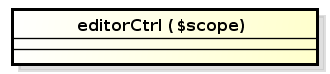
\includegraphics[scale=0.80]{img/diacla/editorCtrl.png}
\caption{Diagramma della classe premi/client/editor/controllers/editorCtrl}
\end{center}
\end{figure}

\begin{description}
%-------  descrizione della classe%
\item[Descrizione] \hfill
	Questo controller non è al momento provvisto di funzionalità. Si appoggia alla vista associata \textit{editor.ng}, la quale funge da scheletro per le viste necessarie alla gestione dei vari editor a disposizione dell'utente. 
\end{description}

%-------  diagramma della classe%
\subsubsection{premi/client/editor/controllers/basicToolbarCtrl}
\begin{figure}[H]
\begin{center}
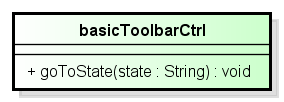
\includegraphics[scale=0.85]{img/diacla/basicToolbarCtrl.png}
\caption{Diagramma della classe premi/editor/controllers/basicToolbarCtrl}
\end{center}
\end{figure}


\begin{description}
%-------  descrizione della classe%
\item[Descrizione] \hfill
	Controller della view \textit{basicToolbar.ng}. Fornisce, tramite lo \textit{\$scope} un metodo per passaggio da un editor all'altro
	\\ La dicitura \{\$scope\} nel diagramma UML$_G$ indica che:
\begin{itemize}
\item tutti gli attributi e i metodi pubblici del controller vanno inseriti nello \$scope;
\item tutti gli attributi e i metodi privati del controller appartengono al controller.
\end{itemize}
Vedere la sezione \ref{servizi} per approfondimenti sull'oggetto \$scope.
	
%-------  lista dei metodi%	
\item[Metodi] \hfill

	% -- inizio metodo -- %
	\begin{description}
		\item[\textbf{\color{blue}+ goToState(state : String) : void			}] \hfill
			Tramite il metodo \textit{\$state.go} cambia "stato" dell'editor, passando da una fase di creazione della presentazione all'altra.
			
		\begin{description}
			% -- lista argomenti del metodo -- %
			\item[Argomenti] \hfill
				\begin{itemize}
				
					\item \textbf{state : String			} \hfill
					Il nuovo stato dell'editor. Gli stati dell'editor al momento sono:
					\begin{itemize}
						\item "premi.editor.frame"
						\item "premi.editor.infographic"
						\item "premi.editor.trails"
					\end{itemize}
					
				\end{itemize}
		\end{description}
	\end{description}
	% -- fine metodo -- %
	
	% -- inizio metodo -- %
	\begin{description}
		\item[\textbf{\color{blue}+ activeStateClass(state : String) : String			}] \hfill
			Verifica se un determinato stato è attivo. Restituisce "active" nel caso lo stato sia attivo altrimenti restituisce una stringa vuota.
			
		\begin{description}
			% -- lista argomenti del metodo -- %
			\item[Argomenti] \hfill
				\begin{itemize}
				
					\item \textbf{state : String			} \hfill
					identifica il nome dello stato da controllare.
					
				\end{itemize}
		\end{description}
	\end{description}
	% -- fine metodo -- %	
		
\end{description}


\subsubsection{premi/client/editor/lib/GObject}
\begin{figure}[H]
\begin{center}
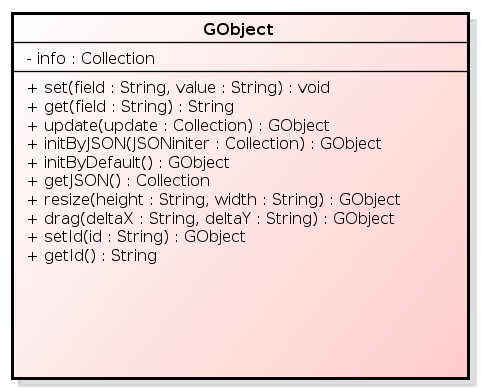
\includegraphics[scale=0.80]{img/diacla/GObject.png}
\caption{Diagramma della classe premi/client/editor/lib/GObject}
\end{center}
\end{figure}

\begin{description}
%-------  descrizione della classe%
\item[Descrizione] \hfill
	GObject è una classe astratta che rappresenta un oggetto generico della presentazione. Contiene i metodi generali che caratterizzano ciascun oggetto grafico che può essere inserito in una presentazione.
	
%-------  lista degli Attributi%	
\item[Attributi] \hfill
	\begin{description}
		\item[\textbf{- info : Collection			}] \hfill
			info è un oggetto JSON che contiene i seguenti campi:
				\begin{itemize}
					\item \textit{\_id:} rappresenta l'id che identifica l'oggetto;
					\item \textit{dataX:} identifica la posizione orizzontale dell'asse x dell'oggetto;
					\item \textit{dataY:} identifica la posizione verticale dell'asse y dell'oggetto;
					\item \textit{dataZ:} identifica il grado di trasparenza dell'oggetto; %da chiedere%
					\item \textit{height:} identifica l'altezza dell'oggetto;
					\item \textit{width:} identifica la larghezza dell'oggetto;
					\item \textit{scale:} identifica la scala dell'oggetto; %da chiedere%
					\item \textit{lvl:} identifica il livello dell'oggetto. %da chiedere%
				\end{itemize}
			
			Viene inizializzato dal metodo initByDefault e il seguente è l'oggetto JSON inizializzato con i valori di default:
\begin{lstlisting}
{
    "_id"               : "",
    "dataX"             : 0,
    "dataY"             : 0,
    "dataZ"             : 0,
    "height"            : 100,
    "width"             : 100,
    "scale"             : 1,
    "lvl"               : 0
}
\end{lstlisting}					
                 L'attributo Info è usato in molti metodi di questa classe. Ad ogni metodo che si interfaccia con questo oggetto, verrà specificato nella descrizione le modifiche che vengono apportate. 
		
	\end{description}
	
	
%-------  lista dei metodi
\item[Metodi] \hfill

	% -- inizio metodo -- %
	\begin{description}
		\item[\textbf{\color{blue}+ set(field : String, value : String) : GObject			}] \hfill
			permette di settare un campo dell'attributo info. Restituisce un riferimento di GObject.
			
		\begin{description}
			% -- lista argomenti del metodo -- %
			\item[Argomenti] \hfill
				\begin{itemize}
				
					\item \textbf{field : String			} \hfill
					field identifica il campo da settare di info;
					\item \textbf{value : String			} \hfill
					value rappresenta il valore del campo da settare su l'attributo info.
				\end{itemize}
		\end{description}-

\end{description}

\begin{description}
		\item[\textbf{\color{blue}+ get(field : String) : String			}] \hfill
			restituisce il valore di un campo dell'attributo info. Restituisce un valore del campo info richiesto.
			
		\begin{description}
			% -- lista argomenti del metodo -- %
			\item[Argomenti] \hfill
				\begin{itemize}
				
					\item \textbf{field : String			} \hfill
					field identifica l'attributo info di cui si vuole venga restituito il valore.
				\end{itemize}
		\end{description}

\end{description}

\begin{description}
		\item[\textbf{\color{blue}+ update(update : Collection) : GObject			}] \hfill
			permette di aggiornare i campi dell'attributo info. Restituisce un riferimento di GObject.
			
		\begin{description}
			% -- lista argomenti del metodo -- %
			\item[Argomenti] \hfill
				\begin{itemize}
				
					\item \textbf{update : Collection			} \hfill
					update è un oggetto JSON che contiene chiave e valore dei campi che devono essere aggiornati. 
				\end{itemize}
		\end{description}

\end{description}

\begin{description}
		\item[\textbf{\color{blue}+ initByJSON(JSONiniter : Collection) : Gobject			}] \hfill
			permette di inizializzare l'attributo info tramite un oggetto JSON. Restituisce un riferimento di GObject. 
			
		\begin{description}
			% -- lista argomenti del metodo -- %
			\item[Argomenti] \hfill
				\begin{itemize}
				
					\item \textbf{JSONiniter : Collection			} \hfill
					è un oggetto JSON che contiene chiave e valore di inizializzazione dei campi dell'attributo info. 
				\end{itemize}
		\end{description}

\end{description}

\begin{description}
		\item[\textbf{\color{blue}+ initByDefault() : GObject			}] \hfill
			permette di inizializzare i campi dell'attributo info con i parametri di default. Restituisce un riferimento di GObject.

\end{description}

\begin{description}
		\item[\textbf{\color{blue}+ getJSON() : String			}] \hfill
			restituisce la collection dell'attributo info.

\end{description}

\begin{description}
		\item[\textbf{\color{blue}+ resize(height : String, width : String) : GObject			}] \hfill
			permette di settare l'altezza e la larghezza del'oggetto. Restituisce un riferimento di GObject.
			
		\begin{description}
			% -- lista argomenti del metodo -- %
			\item[Argomenti] \hfill
				\begin{itemize}
				
					\item \textbf{height : String			} \hfill
					identifica il valore dell'altezza da settare sul campo height dell'attributo info;
					\item \textbf{width : String			} \hfill
					identifica il valore dell'altezza da settare sul campo width dell'attributo info;				
				\end{itemize}
		\end{description}
		
\end{description}

\begin{description}
		\item[\textbf{\color{blue}+ drag(deltaX : String, deltaY : String) : GObject			}] \hfill
			permette di settare la posizione dell'oggetto sull'asse x e y. Restituisce un riferimento di GObject.
			
		\begin{description}
			% -- lista argomenti del metodo -- %
			\item[Argomenti] \hfill
				\begin{itemize}
				
					\item \textbf{deltaX : String			} \hfill
					identifica il valore della posizione sull'asse x da settare sul campo deltaX dell'attributo info.
					\item \textbf{deltaY : String			} \hfill
					identifica il valore della posizione sull'asse y da settare sul campo deltaY dell'attributo info;				
				\end{itemize}
		\end{description}
		
\end{description}

\begin{description}
		\item[\textbf{\color{blue}+ setId(id : String) : GObject			}] \hfill
			permette di modificare o di settare l'id dell'oggetto. Restituisce un riferimento di GObject.
			
		\begin{description}
			% -- lista argomenti del metodo -- %
			\item[Argomenti] \hfill
				\begin{itemize}
				
					\item \textbf{id : String			} \hfill
					identifica il valore dell'id da settare sul campo \_id dell'attributo info.
				\end{itemize}
		\end{description}
		
\end{description}

\begin{description}
		\item[\textbf{\color{blue}+ getId() : String			}] \hfill
			restituisce l'id dell'oggetto.
\end{description}


\end{description}

\subsubsection{premi/client/editor/lib/GOProvider}
\begin{figure}[H]
\begin{center}
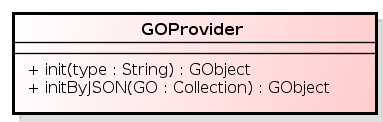
\includegraphics[scale=0.90]{img/diacla/GOProvider.png}
\caption{Diagramma della classe premi/client/editor/lib/GOProvider}
\end{center}
\end{figure}

\begin{description}
%-------  descrizione della classe%
\item[Descrizione] \hfill
	E' una classe statica contiene i metodi per inizializzare gli oggetti image, text, shape che possono essere inseriti in un frame.
	
	\item[Dipendenze] \hfill
	\begin{itemize}
		\item \textbf{Image}: per inizializzare le immagini;
		\item \textbf{Shape}: per inizializzare gli shape;
		\item \textbf{Text}: per inizializzare i testi.
	\end{itemize}
	
%-------  lista dei metodi
\item[Metodi] \hfill

	% -- inizio metodo -- %
	\begin{description}
		\item[\textbf{\color{blue}+ init(type : String) : Collection			}] \hfill
			inizializza con i parametri di default un oggetto image, shape o text e restituisce un oggetto JSON che contiene tutti i campi dell'attributo info dell'oggetto (image, shape, text) a cui si riferisce. Ad esempio se init inizializza un oggetto text restituisce un JSON con le seguenti coppie chiave - valore:
\begin{lstlisting}
{
    "_id"               : "",
    "dataX"             : 0,
    "dataY"             : 0,
    "dataZ"             : 0,
    "height"            : 100,
    "width"             : 100,
    "scale"             : 1,
    "lvl"               : 0,
    "text"              : "text",
    "type"              : "text",
    "color"             : "#ffffff",
    "weight"            : "",
    "fontStyle"         : "",
    "textDecoration"    : "",
    "sizeFontText"      : 20,
    "fontFamily"        : "Arial"
}
\end{lstlisting}
			
		\begin{description}
			% -- lista argomenti del metodo -- %
			\item[Argomenti] \hfill
				\begin{itemize}
				
					\item \textbf{type : String			} \hfill
					identifica il tipo di oggetto da inizializzare.
				\end{itemize}
		\end{description}

\end{description}

	% -- inizio metodo -- %
	\begin{description}
		\item[\textbf{\color{blue}+ initByJSON(GO : Collection) : Collection			}] \hfill
			inizializza con un oggetto JSON, un oggetto image, text o shape e ne restituisce il riferimento.
			
		\begin{description}
			% -- lista argomenti del metodo -- %
			\item[Argomenti] \hfill
				\begin{itemize}
				
					\item \textbf{GO : Collection			} \hfill
					è un oggetto JSON che serve per inizializzare l'oggetto da resituire come riferimento.
				\end{itemize}
		\end{description}

\end{description}

\end{description}

\subsubsection{premi/client/editor/lib/Frame}
\begin{figure}[H]
\begin{center}
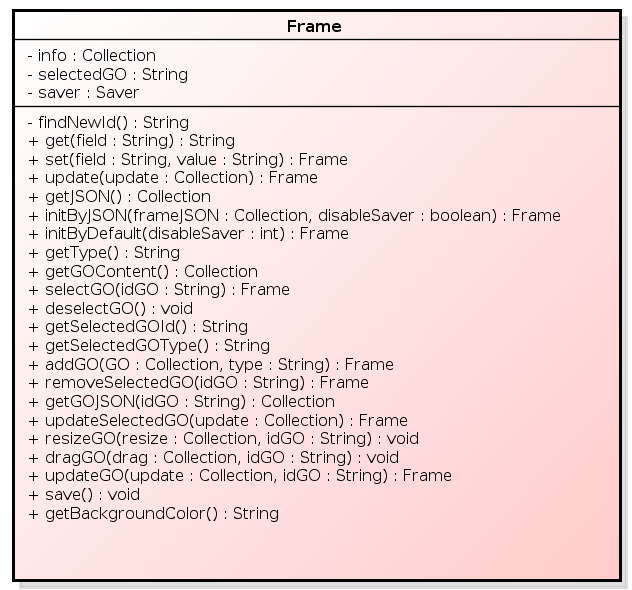
\includegraphics[scale=0.80]{img/diacla/frame.png}
\caption{Diagramma della classe premi/client/editor/lib/Frame}
\end{center}
\end{figure}

\begin{description}
%-------  descrizione della classe%
\item[Descrizione] \hfill
	frame è una classe che rappresenta un frame di una presentazione. E' un oggetto che può essere rappresentato nella presentazione. Per inizializzare gli oggetti image, shape, text si utilizzano i metodi di GOProvider \textit{initByJSON(GO)} e \textit{init(type)}
	
%-------  lista delle classi ereditate%	
\item[Classi ereditate] \hfill
	\begin{itemize}
		\item GObject
	\end{itemize}

\item[Dipendenze] \hfill
	\begin{itemize}
		\item \textbf{GOProvider}: per inizializzare gli oggetti image, shape e text;
		\item \textbf{Saver}: per effettuare le modifiche del frame nel database.
	\end{itemize}

%-------  lista degli Attributi%	
\item[Attributi] \hfill
	\begin{description}
		\item[\textbf{- info : Collection			}] \hfill
			l'attributo info è un oggetto JSON che estende l'attributo info ereditato da GObject. I campi aggiuntivi sono:
	\begin{itemize}
		\item \textit{backgroundColor:} rappresenta il colore di Background del frame;
		\item \textit{content:} è un oggetto JSON che contiene gli oggetti che fanno parte del frame;
		\item \textit{type:} identifica che l'oggetto trattato è un frame.
	\end{itemize}
	
	Viene inizializzato dal metodo initByDefault e il seguente è l'oggetto JSON inizializzato con i valori di default:
\begin{lstlisting}
{
    "_id"               : "",
    "dataX"             : 0,
    "dataY"             : 0,
    "dataZ"             : 0,
    "height"            : 100,
    "width"             : 100,
    "scale"             : 1,
    "lvl"               : 0,
    "backgrooundColor"  : "#ffffff",
    "content"           : {},
    "type"              : "frame"
}
\end{lstlisting}					
                 L'attributo Info è usato in molti metodi di questa classe. Ad ogni metodo che si interfaccia con questo oggetto, verrà specificato nella descrizione le modifiche che vengono apportate. 	
	
	\end{description}
	\begin{description}
		\item[\textbf{- selectedGO : Collection			}] \hfill
			contiene l'oggetto GObject contenuto nel frame corrente selezionato dall'utente.  
	\end{description}
	\begin{description}
		\item[\textbf{- saver : Saver			}] \hfill
			contiene un oggetto saver che permette di interfacciarsi con il database.  
	\end{description}
	
%-------  lista dei metodi
\item[Metodi] \hfill

	% -- inizio metodo -- %
	\begin{description}
		\item[\textbf{\color{blue}- findNewId() : String			}] \hfill
			trova un nuovo id valido per il frame corrente.

\end{description}

	% -- inizio metodo -- %
	\begin{description}
		\item[\textbf{\color{blue}+ set(field : String, value : String) : void			}] \hfill
			permette di settare un campo dell'attributo info.
			
		\begin{description}
			% -- lista argomenti del metodo -- %
			\item[Argomenti] \hfill
				\begin{itemize}
				
					\item \textbf{field : String			} \hfill
					field identifica il campo da settare di info;
					\item \textbf{value : String			} \hfill
					value rappresenta il valore del campo da settare su l'attributo info.
				\end{itemize}
		\end{description}

\end{description}

\begin{description}
		\item[\textbf{\color{blue}+ get(field : String) : String			}] \hfill
			restituisce il valore di un campo dell'attributo info.
			
		\begin{description}
			% -- lista argomenti del metodo -- %
			\item[Argomenti] \hfill
				\begin{itemize}
				
					\item \textbf{field : String			} \hfill
					field identifica l'attributo info di cui si vuole venga restituito il valore.
				\end{itemize}
		\end{description}

\end{description}

\begin{description}
		\item[\textbf{\color{blue}+ update(update : Collection) : Frame			}] \hfill
			permette di aggiornare i campi dell'attributo info. Restituisce un riferimento di Frame.
			
		\begin{description}
			% -- lista argomenti del metodo -- %
			\item[Argomenti] \hfill
				\begin{itemize}
				
					\item \textbf{update : Collection			} \hfill
					update è un oggetto JSON che contiene chiave e valore dei campi che devono essere aggiornati. 
				\end{itemize}
		\end{description}

\end{description}

\begin{description}
		\item[\textbf{\color{blue}+ initByJSON(frameJSON : Collection, disableSaver: boolean) : Frame			}] \hfill
			permette di inizializzare l'attributo info tramite un oggetto JSON. Se disableSaver è uguale a false viene utilizzato il metodo di Saver \textit{setContainer(id,type)} e \textit{init()} per impostare il frame come contenitore per il salvataggio dei dati sul database. Restituisce un riferimento di Frame.
			
		\begin{description}
			% -- lista argomenti del metodo -- %
			\item[Argomenti] \hfill
				\begin{itemize}
				
					\item \textbf{frameJSON : Collection			} \hfill
					è un oggetto JSON che contiene chiave e valore di inizializzazione dei campi dell'attributo info. 
					\item \textbf{disableSaver : boolean			} \hfill
					se è uguale a false il contenuto di frame non viene salvato.  				
				\end{itemize}
		\end{description}

\end{description}

\begin{description}
		\item[\textbf{\color{blue}+ initByDefault(disableSaver) : Frame			}] \hfill
			permette di inizializzare i campi dell'attributo info con i parametri di default. Se disableSaver è uguale a false viene utilizzato il metodo di Saver \textit{setContainer(id,type)} e \textit{init()} per impostare il frame come contenitore per il salvataggio dei dati sul database. Restituisce un riferimento di Frame.

\begin{description}
			% -- lista argomenti del metodo -- %
			\item[Argomenti] \hfill
				\begin{itemize}
						\item \textbf{disableSaver : boolean			} \hfill
					se è uguale a false il contenuto di frame non viene salvato. %da chiedere%  				
				\end{itemize}

\end{description}

\begin{description}
		\item[\textbf{\color{blue}+ getJSON() : String			}] \hfill
			restituisce la collection dell'attributo info.

\end{description}

\begin{description}
		\item[\textbf{\color{blue}+ getType() : String			}] \hfill
			restituisce la stringa "frame" per indicare che il tipo dell'oggetto è frame.
\end{description}

\begin{description}
		\item[\textbf{\color{blue}+ getGOContent() : Collection			}] \hfill
			restituisce il contenuto della collezione content che è un insieme di oggetti JSON che fanno parte del frame.
\end{description}

\begin{description}
		\item[\textbf{\color{blue}+ selectGO(idGO) : Collection			}] \hfill
			restituisce l'oggetto grafico con id = idGO contenuto all'interno del frame. 

\begin{description}
			% -- lista argomenti del metodo -- %
			\item[Argomenti] \hfill
				\begin{itemize}
						\item \textbf{idGO : String			} \hfill
					valore dell'id dell'oggetto grafico da restituire.  				
				\end{itemize}

\end{description}

\end{description}

\begin{description}
		\item[\textbf{\color{blue}+ deselectGO() : void			}] \hfill
			deseleziona l'oggetto grafico portando a null l'attributo selectedGo. 
\end{description}

\begin{description}
		\item[\textbf{\color{blue}+ getSelectedGOId() : String			}] \hfill
			restituisce l'id dell'oggetto grafico selezionato.
\end{description}

\begin{description}
		\item[\textbf{\color{blue}+ getSelectedGOType() : String			}] \hfill
			restituisce il tipo dell'oggetto grafico selezionato.
\end{description}

\begin{description}
		\item[\textbf{\color{blue}+ getSelectedGO() : String			}] \hfill
			restituisce l'oggetto grafico selezionato.
\end{description}

\begin{description}
		\item[\textbf{\color{blue}+ addGO(GO : Collection, type : String) : Frame			}] \hfill
			aggiunge un oggetto di tipo type al frame e restituisce il riferimento del frame. Per  salvare sul database viene usato il metodo di Saver \textit{insert(GOJSON)} che permette di appendere un operazione di inserimento nell'oggetto Saver. Restituisce un riferimento di Frame.  

\begin{description}
			% -- lista argomenti del metodo -- %
			\item[Argomenti] \hfill
				\begin{itemize}
						\item \textbf{GO : Collection			} \hfill
					un oggetto JSON che serve per inizializzare l'oggetto da aggiungere al frame;
					  	\item \textbf{type : String			} \hfill
					  	contiene il tipo dell'oggetto da inserire nel frame.
				\end{itemize}

\end{description}

\end{description}


\begin{description}
		\item[\textbf{\color{blue}+ removeSelectedGO(idGO : String) : Frame			}] \hfill
			se l'oggetto con id = idGO è selezionato lo elimina. Viene utilizzato il metodo \textit{remove(idGO,type)} che permette di appendere un operazione di rimozione nell'oggetto Saver. Restituisce un riferimento di Frame.

\begin{description}
			% -- lista argomenti del metodo -- %
			\item[Argomenti] \hfill
				\begin{itemize}
						\item \textbf{idGO : Collection			} \hfill
						rappresenta l'id dell'oggetto da eliminare.
				\end{itemize}

\end{description}

\end{description}


\begin{description}
		\item[\textbf{\color{blue}+ getGOJSON(idGO : String) : Collection			}] \hfill
			restituisce l'oggetto JSON con id= idGO appartenente al frame.   

\begin{description}
			% -- lista argomenti del metodo -- %
			\item[Argomenti] \hfill
				\begin{itemize}
						\item \textbf{idGO : String			} \hfill
					contiene l'id dell'oggetto che dev'essere restituito.
				\end{itemize}

\end{description}

\end{description}

\begin{description}
		\item[\textbf{\color{blue}+ updateSelectedGO(update : Collection) : Collection			}] \hfill
			aggiorna i campi dell'oggetto selezionato.   

\begin{description}
			% -- lista argomenti del metodo -- %
			\item[Argomenti] \hfill
				\begin{itemize}
						\item \textbf{update : Collection			} \hfill
					è un oggetto JSON che contiene chiave e valore dei campi da aggiornare dell'oggetto selezionato. Viene utilizzato il metodo \textit{update(idGO,type,update)} per appendere un operazione di modifica nell'oggetto Saver.
				\end{itemize}

\end{description}

\end{description}

\begin{description}
		\item[\textbf{\color{blue}+ resizeGO(resize : Collection, idGO : String) : void			}] \hfill
			aggiorna i campi dell'oggetto con un determinato id, per permettere il ridimensionamento dell'oggetto. Viene utilizzato il metodo \textit{update(idGO,type,update)} per appendere le operazioni di modifica nell'oggetto Saver.    

\begin{description}
			% -- lista argomenti del metodo -- %
			\item[Argomenti] \hfill
				\begin{itemize}
					\item \textbf{resize : Collection			} \hfill
					è un oggetto JSON che contiene chiave e valore dei campi height, width, dataX e dataY per permettere di ridimensionare l'oggetto appartenente al frame;
					\item \textbf{idGO : String			} \hfill
					contiene l'id dell'oggetto da ridimensionare.
				\end{itemize}

\end{description}

\end{description}

\begin{description}
		\item[\textbf{\color{blue}+ dragGO(drag : Collection, idGO : String) : void			}] \hfill
			aggiorna i campi dell'oggetto con un determinato id, per permettere lo spostamento dell'oggetto nel template grafico. Viene utilizzato il metodo \textit{update(idGO,type,update)} per appendere le operazioni di modifica nell'oggetto Saver.    

\begin{description}
			% -- lista argomenti del metodo -- %
			\item[Argomenti] \hfill
				\begin{itemize}
					\item \textbf{drag : Collection			} \hfill
					è un oggetto JSON che contiene chiave e valore dei campi dataX e dataY per permettere lo spostamento dell'oggetto appartenente al frame;
					\item \textbf{idGO : String			} \hfill
					contiene l'id dell'oggetto da spostare.
				\end{itemize}

\end{description}

\end{description}

\begin{description}
		\item[\textbf{\color{blue}+ updateGO(update : Collection, idGO : String) : void			}] \hfill
			aggiorna i campi dell'oggetto con un determinato id appartenente al frame. Viene utilizzato il metodo \textit{update(idGO,type,update)} per appendere un operazione di modifica nell'oggetto Saver. 

\begin{description}
			% -- lista argomenti del metodo -- %
			\item[Argomenti] \hfill
				\begin{itemize}
						\item \textbf{update : Collection			} \hfill
					è un oggetto JSON che contiene chiave e valore dei campi da aggiornare dell'oggetto con un determinato id;
					\item \textbf{idGO : String			} \hfill
					contiene l'id dell'oggetto da aggiornare.
				\end{itemize}

\end{description}

\end{description}

\begin{description}
		\item[\textbf{\color{blue}+ save() : void			}] \hfill
			salva le operazioni pendenti nel database. Viene utilizzato il metodo \textit{save()} che si occupa di inserire le operazioni di inserimento, modifica, rimozione presenti nell'oggetto Saver nel database. 

\end{description}

\begin{description} 
		\item[\textbf{\color{blue}+ getBackgroundColor() : String			}] \hfill
			restituisce il colore in formato esadecimale dello sfondo del frame.     

\end{description}



\end{description}

\end{description}


\subsubsection{premi/client/editor/lib/GOContainer}
\begin{figure}[H]
\begin{center}
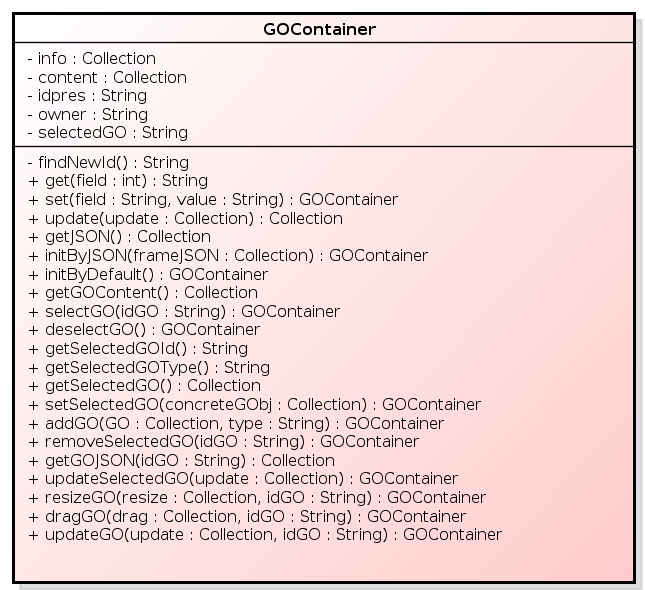
\includegraphics[scale=0.80]{img/diacla/GOContainer.png}
\caption{Diagramma della classe premi/client/editor/lib/GOContainer}
\end{center}
\end{figure}

\begin{description}
%-------  descrizione della classe%
\item[Descrizione] \hfill
	è una classe che rappresenta il contenitore degli oggetti che possono essere inseriti in un frame. Per inizializzare gli oggetti image, shape, text si utilizzano i metodi di GOProvider \textit{initByJSON(GO)} e \textit{init(type)}. 
	
	\item[Classi ereditate] \hfill
	\begin{itemize}
		\item GObject
	\end{itemize}
	
	\item[Dipendenze] \hfill
	\begin{itemize}
		\item \textbf{GOProvider}: per inizializzare gli oggetti image, shape e text.
	\end{itemize}
	
%-------  lista degli Attributi%	
\item[Attributi] \hfill
	\begin{description}
		\item[\textbf{- info : Collection			}] \hfill
			l'attributo info è un oggetto JSON che estende l'attributo info ereditato da GObject. I campi aggiuntivi sono:
	\begin{itemize}
		\item \textit{background:} è un oggetto JSON che contiene i seguenti campi:
		\begin{itemize}
			\item \textit{image:} definisce il percorso dell'immagine di background;
			\item \textit{size:} definisce la grandezza dell'immagine di background;
			\item \textit{color:} definisce il colore di background;
			\item \textit{repeat:} definisce il metodo di ripetizione dello sfondo di background;
			\item \textit{type:} definisce il nome del tipo dell'oggetto.
		\end{itemize}		
		\item \textit{content:} è un oggetto JSON che contiene gli oggetti che fanno parte del frame;
		\item \textit{idpres:} identifica l'id della presentazione a cui si riferisce;
		\item \textit{owner:} identifica l'id dell'utente che ha creato la presentazione.
	\end{itemize}
	Viene inizializzato dal metodo initByDefault e il seguente è l'oggetto JSON inizializzato con i valori di default:
\begin{lstlisting}
{
    "_id"               : "",
    "dataX"             : 0,
    "dataY"             : 0,
    "dataZ"             : 0,
    "height"            : 100,
    "width"             : 100,
    "scale"             : 1,
    "lvl"               : 0,
    "background" {
          image : "",
          size  : "cover",
          color : "antiquewhite",
          repeat: "no-repeat"
                 }
    "content"           : {},
    "presid"            : "",
    "owner"             : "",
    "type"              : ""
}
\end{lstlisting}					
                 L'attributo Info è usato in molti metodi di questa classe. Ad ogni metodo che si interfaccia con questo oggetto, verrà specificato nella descrizione le modifiche che vengono apportate.
	\end{description}
	\begin{description}
		\item[\textbf{- selectedGO : GObject			}] \hfill
			contiene l'oggetto GObject contenuto nel frame corrente selezionato dall'utente.  
	\end{description}
	
%-------  lista dei metodi
\item[Metodi] \hfill

\begin{description}
		\item[\textbf{\color{blue}- findNewId() : String			}] \hfill
			trova un nuovo id valido per il frame corrente.

\end{description}

	% -- inizio metodo -- %
	\begin{description}
		\item[\textbf{\color{blue}+ set(field : String, value : String) : void			}] \hfill
			permette di settare un campo dell'attributo info.
			
		\begin{description}
			% -- lista argomenti del metodo -- %
			\item[Argomenti] \hfill
				\begin{itemize}
				
					\item \textbf{field : String			} \hfill
					field identifica il campo da settare di info;
					\item \textbf{value : String			} \hfill
					value rappresenta il valore del campo da settare su l'attributo info.
				\end{itemize}
		\end{description}

\end{description}

\begin{description}
		\item[\textbf{\color{blue}+ get(field : String) : String			}] \hfill
			restituisce il valore di un campo dell'attributo info.
			
		\begin{description}
			% -- lista argomenti del metodo -- %
			\item[Argomenti] \hfill
				\begin{itemize}
				
					\item \textbf{field : String			} \hfill
					field identifica l'attributo info di cui si vuole venga restituito il valore.
				\end{itemize}
		\end{description}

\end{description}

\begin{description}
		\item[\textbf{\color{blue}+ update(update : Collection) : GOContainer			}] \hfill
			permette di aggiornare i campi dell'attributo info. Restituisce un riferimento di GOContainer.
			
		\begin{description}
			% -- lista argomenti del metodo -- %
			\item[Argomenti] \hfill
				\begin{itemize}
				
					\item \textbf{update : Collection			} \hfill
					update è un oggetto JSON che contiene chiave e valore dei campi che devono essere aggiornati. 
				\end{itemize}
		\end{description}

\end{description}

\begin{description}
		\item[\textbf{\color{blue}+ initByJSON(frameJSON : Collection, disableSaver: boolean) : frame			}] \hfill
			permette di inizializzare l'attributo info tramite un oggetto JSON. 
			
		\begin{description}
			% -- lista argomenti del metodo -- %
			\item[Argomenti] \hfill
				\begin{itemize}
				
					\item \textbf{frameJSON : Collection			} \hfill
					è un oggetto JSON che contiene chiave e valore di inizializzazione dei campi dell'attributo info. 
					\item \textbf{disableSaver : boolean			} \hfill
					se è uguale a false il contenuto di frame non viene salvato. %da chiedere%  				
				\end{itemize}
		\end{description}

\end{description}

\begin{description}
		\item[\textbf{\color{blue}+ initByDefault(disableSaver) : GOContainer			}] \hfill
			permette di inizializzare i campi dell'attributo info con i parametri di default. Restituisce un riferimento di GOContainer. 

\begin{description}
			% -- lista argomenti del metodo -- %
			\item[Argomenti] \hfill
				\begin{itemize}
						\item \textbf{disableSaver : boolean			} \hfill
					se è uguale a false il contenuto di frame non viene salvato. %da chiedere%  				
				\end{itemize}

\end{description}

\end{description}

\begin{description}
		\item[\textbf{\color{blue}+ getGOContent() : Collection			}] \hfill
			restituisce il contenuto della collezione content che è un insieme di oggetti JSON che fanno parte del frame.
\end{description}

\begin{description}
		\item[\textbf{\color{blue}+ selectGO(idGO) : GObject			}] \hfill
			restituisce l'oggetto grafico con id = idGO contenuto all'interno del GOContainer. 

\begin{description}
			% -- lista argomenti del metodo -- %
			\item[Argomenti] \hfill
				\begin{itemize}
						\item \textbf{idGO : String			} \hfill
					valore dell'id dell'oggetto grafico da restituire.  				
				\end{itemize}

\end{description}

\end{description}

\begin{description}
		\item[\textbf{\color{blue}+ deselectGO() : void			}] \hfill
			deseleziona l'oggetto grafico portando a null l'attributo selectedGo. 
\end{description}

\begin{description}
		\item[\textbf{\color{blue}+ getSelectedGOId() : String			}] \hfill
			restituisce l'id dell'oggetto grafico selezionato.
\end{description}

\begin{description}
		\item[\textbf{\color{blue}+ getSelectedGOType() : String			}] \hfill
			restituisce il tipo dell'oggetto grafico selezionato.
\end{description}

\begin{description}
		\item[\textbf{\color{blue}+ getSelectedGO() : String			}] \hfill
			restituisce l'oggetto grafico selezionato.
\end{description}

\begin{description}
		\item[\textbf{\color{blue}+ setSelectedGO(concreteGObj : Collection) : frame			}] \hfill
			setta l'oggetto concreteGObj come oggetto selezionato.  

\begin{description}
			% -- lista argomenti del metodo -- %
			\item[Argomenti] \hfill
				\begin{itemize}
						\item \textbf{concreteGObj : Collection			} \hfill
					oggetto GObject.
				\end{itemize}

\end{description}

\end{description}

\begin{description}
		\item[\textbf{\color{blue}+ addGO(GO : Collection, type : String) : GOContainer			}] \hfill
			aggiunge un oggetto di tipo type al GOContainer e restituisce il riferimento del GOContainer.  

\begin{description}
			% -- lista argomenti del metodo -- %
			\item[Argomenti] \hfill
				\begin{itemize}
						\item \textbf{GO : Collection			} \hfill
					un oggetto JSON che serve per inizializzare l'oggetto da aggiungere al GOContainer;
					  	\item \textbf{type : String			} \hfill
					  	contiene il tipo dell'oggetto da inserire nel GOContainer.
				\end{itemize}

\end{description}

\end{description}

\begin{description}
		\item[\textbf{\color{blue}+ removeSelectedGO(idGO : String) : GOContainer			}] \hfill
			se l'oggetto con id = idGO è selezionato lo elimina. Restituisce un riferimento di GOContainer. 

\begin{description}
			% -- lista argomenti del metodo -- %
			\item[Argomenti] \hfill
				\begin{itemize}
						\item \textbf{idGO : Collection			} \hfill
					rappresenta l'id dell'oggetto da eliminare.
				\end{itemize}

\end{description}

\end{description}


\begin{description}
		\item[\textbf{\color{blue}+ getGOJSON(idGO : String) : Collection			}] \hfill
			restituisce l'oggetto JSON con id= idGO appartenente al GOContainer.   

\begin{description}
			% -- lista argomenti del metodo -- %
			\item[Argomenti] \hfill
				\begin{itemize}
						\item \textbf{idGO : String			} \hfill
					contiene l'id dell'oggetto che dev'essere restituito.
				\end{itemize}

\end{description}

\end{description}

\begin{description}
		\item[\textbf{\color{blue}+ updateSelectedGO(update : Collection) : Collection			}] \hfill
			aggiorna i campi dell'oggetto selezionato.   

\begin{description}
			% -- lista argomenti del metodo -- %
			\item[Argomenti] \hfill
				\begin{itemize}
						\item \textbf{update : Collection			} \hfill
					è un oggetto JSON che contiene chiave e valore dei campi da aggiornare dell'oggetto selezionato.
				\end{itemize}

\end{description}

\end{description}

\begin{description}
		\item[\textbf{\color{blue}+ resizeGO(resize : Collection, idGO : String) : void			}] \hfill
			aggiorna i campi dell'oggetto con un determinato id, per permettere il ridimensionamento dell'oggetto.    

\begin{description}
			% -- lista argomenti del metodo -- %
			\item[Argomenti] \hfill
				\begin{itemize}
					\item \textbf{resize : Collection			} \hfill
					è un oggetto JSON che contiene chiave e valore dei campi height, width, dataX e dataY per permettere di ridimensionare l'oggetto appartenente al GOContainer;
					\item \textbf{idGO : String			} \hfill
					contiene l'id dell'oggetto da ridimensionare.
				\end{itemize}

\end{description}

\end{description}

\begin{description}
		\item[\textbf{\color{blue}+ dragGO(drag : Collection, idGO : String) : void			}] \hfill
			aggiorna i campi dell'oggetto con un determinato id, per permettere lo spostamento dell'oggetto nel template grafico.    

\begin{description}
			% -- lista argomenti del metodo -- %
			\item[Argomenti] \hfill
				\begin{itemize}
					\item \textbf{drag : Collection			} \hfill
					è un oggetto JSON che contiene chiave e valore dei campi dataX e dataY per permettere lo spostamento dell'oggetto appartenente al GOContainer;
					\item \textbf{idGO : String			} \hfill
					contiene l'id dell'oggetto da spostare.
				\end{itemize}

\end{description}

\end{description}

\begin{description}
		\item[\textbf{\color{blue}+ updateGO(update : Collection, idGO : String) : void			}] \hfill
			aggiorna i campi dell'oggetto con un determinato id appartenente al GOContainer.  

\begin{description}
			% -- lista argomenti del metodo -- %
			\item[Argomenti] \hfill
				\begin{itemize}
						\item \textbf{update : Collection			} \hfill
					è un oggetto JSON che contiene chiave e valore dei campi da aggiornare dell'oggetto con un determinato id;
					\item \textbf{idGO : String			} \hfill
					contiene l'id dell'oggetto da aggiornare.
				\end{itemize}

\end{description}

\end{description}


\end{description}

\subsubsection{premi/client/editor/lib/Image}
\begin{figure}[H]
\begin{center}
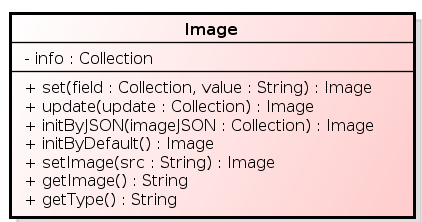
\includegraphics[scale=0.80]{img/diacla/Image.png}
\caption{Diagramma della classe premi/client/editor/lib/Image}
\end{center}
\end{figure}

\begin{description}
%-------  descrizione della classe%
\item[Descrizione] \hfill
	è una classe che rappresenta un oggetto immagine. Contiene i metodi per gestire un immagine.
	
\item[Classi ereditate] \hfill
	\begin{itemize}
		\item GObject
	\end{itemize}
	
%-------  lista degli Attributi%	
\item[Attributi] \hfill
	\begin{description}
		\item[\textbf{- info : Collection			}] \hfill
			l'attributo info è un oggetto JSON che estende l'attributo info ereditato da GObject. I campi aggiuntivi sono:
	\begin{itemize}
		\item \textit{src:} definisce il percorso dell'immagine;
		\item \textit{type:} identifica il tipo di oggetto.		
	\end{itemize}
	Viene inizializzato dal metodo initByDefault e il seguente è l'oggetto JSON inizializzato con i valori di default:
\begin{lstlisting}
{
    "_id"               : "",    
    "dataX"             : 0,
    "dataY"             : 0,
    "dataZ"             : 0,
    "height"            : 100,
    "width"             : 100,
    "scale"             : 1,
    "lvl"               : 0,
    "src"               : "ffff",
    "type"              : "image"
}
\end{lstlisting}					
                 L'attributo Info è usato in molti metodi di questa classe. Ad ogni metodo che si interfaccia con questo oggetto, verrà specificato nella descrizione le modifiche che vengono apportate. 
    \end{description}
	\begin{description}
		\item[\textbf{- selectedGO : Collection			}] \hfill
			contiene l'oggetto GObject contenuto nel frame corrente selezionato dall'utente.  
	\end{description}	
	
%-------  lista dei metodi
\item[Metodi] \hfill

		\begin{description}
		\item[\textbf{\color{blue}+ set(field : String, value : String) : void			}] \hfill
			permette di settare un campo dell'attributo info.
			
		\begin{description}
			% -- lista argomenti del metodo -- %
			\item[Argomenti] \hfill
				\begin{itemize}
				
					\item \textbf{field : String			} \hfill
					identifica il campo da settare di info;
					\item \textbf{value : String			} \hfill
					rappresenta il valore del campo da settare su l'attributo info.
				\end{itemize}
		\end{description}

\end{description}

\begin{description}
		\item[\textbf{\color{blue}+ update(update : Collection) : Image			}] \hfill
			permette di aggiornare i campi dell'attributo info. Restituisce un riferimento di Image.
			
		\begin{description}
			% -- lista argomenti del metodo -- %
			\item[Argomenti] \hfill
				\begin{itemize}
				
					\item \textbf{update : Collection			} \hfill
					update è un oggetto JSON che contiene chiave e valore dei campi che devono essere aggiornati. 
				\end{itemize}
		\end{description}

\end{description}

\begin{description}
		\item[\textbf{\color{blue}+ initByJSON(imageJSON : Collection) : Image			}] \hfill
			permette di inizializzare l'attributo info tramite un oggetto JSON. Restituisce un riferimento di Image.
			
		\begin{description}
			% -- lista argomenti del metodo -- %
			\item[Argomenti] \hfill
				\begin{itemize}
				
					\item \textbf{imageJSON : Collection			} \hfill
					è un oggetto JSON che contiene chiave e valore di inizializzazione dei campi dell'attributo info. 
				\end{itemize}
		\end{description}

\end{description}

\begin{description}
		\item[\textbf{\color{blue}+ initByDefault() : Image			}] \hfill
			permette di inizializzare i campi dell'attributo info con i parametri di default. Restituisce un riferimento di Image. 

\end{description}

\begin{description}
		\item[\textbf{\color{blue}+ setImage(src : String) : Image			}] \hfill
			setta l'url(percorso) dell'immagine. Restituisce un riferimento di Image.
			
		\begin{description}
			% -- lista argomenti del metodo -- %
			\item[Argomenti] \hfill
				\begin{itemize}
				
					\item \textbf{src : String			} \hfill
					identifica l'url(percorso) dell'immagine.
				\end{itemize}
		\end{description}

\end{description}

\begin{description}
		\item[\textbf{\color{blue}+ getImage() : String			}] \hfill
			restituisce l'url(percorso) dell'immagine. 

\end{description}

\begin{description}
		\item[\textbf{\color{blue}+ getType() : String			}] \hfill
			restituisce la stringa "image" per identificare che il tipo dell'oggetto è image. 

\end{description}



\end{description}


\subsubsection{premi/client/editor/lib/Infographic}
\begin{figure}[H]
\begin{center}
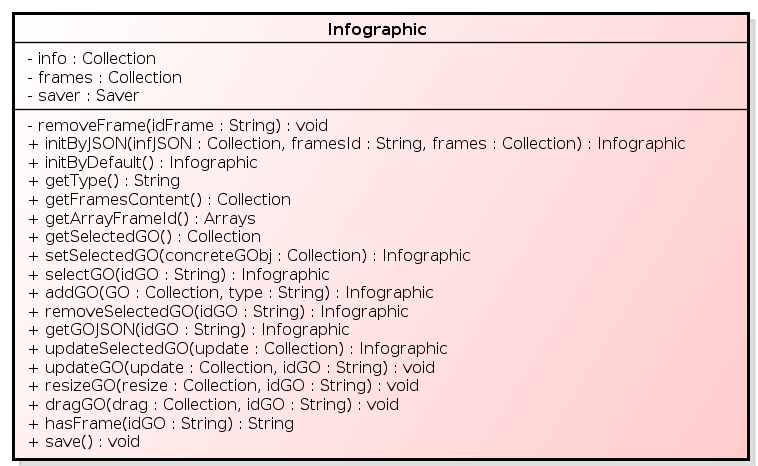
\includegraphics[scale=0.80]{img/diacla/Infographic.png}
\caption{Diagramma della classe premi/client/editor/lib/infographic}
\end{center}
\end{figure}

\begin{description}
%-------  descrizione della classe%
\item[Descrizione] \hfill
	è una classe che rappresenta un oggetto infografica. Un infografica contiene i frame e gli oggetti che si vogliono visualizzare nella presentazione.
	
\item[Classi ereditate] \hfill
	\begin{itemize}
		\item GOContainer
	\end{itemize}
	
\item[Dipendenze] \hfill
	\begin{itemize}
		\item \textbf{Frame}: per gestire i frame nell'infografica;
		\item \textbf{Saver}: per apportare le modifiche sul database.
	\end{itemize}	
	
%-------  lista degli Attributi%	
\item[Attributi] \hfill
	\begin{description}
		\item[\textbf{- info : Collection			}] \hfill
			l'attributo info è un oggetto JSON che estende l'attributo info ereditato da GObject. I campi aggiuntivi sono:
	\begin{itemize}
		\item \textit{framesId:} array che contiene gli id dei frame appartenenti all'infografica;
		\item \textit{type:} identifica il tipo di oggetto ovvero infografica.		
	\end{itemize}
	Viene inizializzato dal metodo initByDefault e il seguente è l'oggetto JSON inizializzato con i valori di default:
\begin{lstlisting}
{
    "_id"               : "",    
    "dataX"             : 0,
    "dataY"             : 0,
    "dataZ"             : 0,
    "height"            : 100,
    "width"             : 100,
    "scale"             : 1,
    "lvl"               : 0,
    "framesId"          : [],
    "type"              : "infographic"
}
\end{lstlisting}					
                 L'attributo Info è usato in molti metodi di questa classe. Ad ogni metodo che si interfaccia con questo oggetto, verrà specificato nella descrizione le modifiche che vengono apportate. 
		\item[\textbf{- frames : Collection			}] \hfill
			contiene degli oggetti JSON che rappresentano i frame appartenenti all'infografica.
		\item[\textbf{- saver : Saver			}] \hfill
			oggetto Saver che si occupa delle modifiche e dei salvataggi su database.
	\end{description}	
	
%-------  lista dei metodi
\item[Metodi] \hfill

		\begin{description}
		\item[\textbf{\color{blue}- removeFrame(idFrame : String) : void			}] \hfill
			rimuove un frame dall'infografica
			
		\begin{description}
			% -- lista argomenti del metodo -- %
			\item[Argomenti] \hfill
				\begin{itemize}
				
					\item \textbf{idFrame : String			} \hfill
						Identifica l'id del frame da rimuovere dall'infografica.
				\end{itemize}
		\end{description}

\end{description}

\begin{description}
		\item[\textbf{\color{blue}+ initByJSON(infJSON : Collection,framesId : String[],frames : Collection) : Infographic			}] \hfill
			permette di inizializzare l'oggetto infografica. Viene utilizzato il metodo \textit{setContainer(id,type)} per selezionare l'oggetto infographic come contenitore dell'oggetto Saver. Restituisce un riferimento di Infographic.
			
		\begin{description}
			% -- lista argomenti del metodo -- %
			\item[Argomenti] \hfill
				\begin{itemize}
				
					\item \textbf{infJSON : Collection			} \hfill
					è un oggetto JSON che contiene chiave e valore di inizializzazione dei campi dell'attributo info;
					\item \textbf{framesId : String[]			} \hfill
					array di identificativi che rappresenta gli id dei frame da aggiungere all'infografica;
					\item \textbf{frames : Collection			} \hfill
					contiene oggetti JSON che identificano i frame appartenenti all'infografica. 
				\end{itemize}
		\end{description}

\end{description}

\begin{description}
		\item[\textbf{\color{blue}+ initByDefault() : Infographic			}] \hfill
			permette di inizializzare i campi dell'attributo info con i parametri di default e di lasciare vuoti l'attributo framesId e frames. Viene utilizzato il metodo \textit{setContainer(id,type)} per selezionare l'oggetto infographic come contenitore dell'oggetto Saver. Restituisce un riferimento di Infographic.

\end{description}

\begin{description}
		\item[\textbf{\color{blue}+ getType() : String			}] \hfill
			restituisce la stringa "infographic" perchè il tipo di oggetto è un infografica.

\end{description}

\begin{description}
		\item[\textbf{\color{blue}+ getFramesContent() : Collection			}] \hfill
			restituisce gli oggetti JSON che rappresentano i frame appartenenti all'infografica.

\end{description}

\begin{description}
		\item[\textbf{\color{blue}+ getArrayFrameId() : Arrays			}] \hfill
			restituisce un array in cui ciascun elemento identifica un frame appartenente all'infografica.

\end{description}

\begin{description}
		\item[\textbf{\color{blue}+ getSelectedGO() : String			}] \hfill
			restituisce l'oggetto selezionato nell'infografica.

\end{description}

\begin{description}
		\item[\textbf{\color{blue}+ setSelectedGO(concreteGObj : Collection) : Infographic			}] \hfill
			imposta su selezionato un oggetto dell'infografica. Restituisce un riferimento di Infographic.

		\begin{description}
			% -- lista argomenti del metodo -- %
			\item[Argomenti] \hfill
				\begin{itemize}
				
					\item \textbf{concreteGObj : Collection			} \hfill
					rappresenta l'oggetto JSON da selezionare nell'infografica.
				\end{itemize}
		\end{description}

\end{description}

\begin{description}
		\item[\textbf{\color{blue}+ selectedGO(idGO : String) : Infographic			}] \hfill
			seleziona un oggetto dell'infografica. Restituisce un riferimento di Infographic.

		\begin{description}
			% -- lista argomenti del metodo -- %
			\item[Argomenti] \hfill
				\begin{itemize}
				
					\item \textbf{idGO : String			} \hfill
					identifica l'id dell'oggetto da selezionare.
				\end{itemize}
		\end{description}

\end{description}

\begin{description}
		\item[\textbf{\color{blue}+ addGO(GO : Collection, type : String) : Infographic			}] \hfill
			aggiunge un oggetto di tipo type all'infografica e restituisce il riferimento dell'infografica. Viene utilizzato il metodo \textit{insert(GOJSON)} di Saver per appendere un operazione di inserimento nell'oggetto saver. Restituisce un riferimento di Infographic. 

\begin{description}
			% -- lista argomenti del metodo -- %
			\item[Argomenti] \hfill
				\begin{itemize}
						\item \textbf{GO : Collection			} \hfill
					un oggetto JSON che serve per inizializzare l'oggetto da aggiungere all'infografica;
					  	\item \textbf{type : String			} \hfill
					  	contiene il tipo dell'oggetto da inserire nell'infografica.
				\end{itemize}

\end{description}

\end{description}


\begin{description}
		\item[\textbf{\color{blue}+ removeSelectedGO(idGO : String) : Infographic			}] \hfill
			se l'oggetto con id = idGO è selezionato lo elimina. Viene utilizzato il metodo \textit{remove(idGO,type)} di Saver per appendere un operazione di rimozione nell'oggetto saver. Restituisce un riferimento di Infographic.

\begin{description}
			% -- lista argomenti del metodo -- %
			\item[Argomenti] \hfill
				\begin{itemize}
						\item \textbf{idGO : Collection			} \hfill
					rappresenta l'id dell'oggetto da eliminare.
				\end{itemize}

\end{description}

\end{description}

\begin{description}
		\item[\textbf{\color{blue}+ getGOJSON(idGO : String) : Collection			}] \hfill
			restituisce l'oggetto JSON con id= idGO appartenente all'infografica.   

\begin{description}
			% -- lista argomenti del metodo -- %
			\item[Argomenti] \hfill
				\begin{itemize}
						\item \textbf{idGO : String			} \hfill
					contiene l'id dell'oggetto che dev'essere restituito.
				\end{itemize}

\end{description}

\end{description}

\begin{description}
		\item[\textbf{\color{blue}+ updateSelectedGO(update : Collection) : Infographic			}] \hfill
			aggiorna i campi dell'oggetto selezionato. Viene utilizzato il metodo \textit{update(idGO,type,update)} di Saver per appendere un operazione di aggiornamento nell'oggetto saver. Restituisce un riferimento di Infographic.  

\begin{description}
			% -- lista argomenti del metodo -- %
			\item[Argomenti] \hfill
				\begin{itemize}
						\item \textbf{update : Collection			} \hfill
					è un oggetto JSON che contiene chiave e valore dei campi da aggiornare dell'oggetto selezionato.
				\end{itemize}

\end{description}

\end{description}

\begin{description}
		\item[\textbf{\color{blue}+ updateGO(update : Collection, idGO : String) : Infographic			}] \hfill
			aggiorna i campi di un oggetto dell'infografica. Viene utilizzato il metodo \textit{update(idGO,type,update)} di Saver per appendere un operazione di aggiornamento nell'oggetto saver. Restituisce un riferimento di Infographic.   

\begin{description}
			% -- lista argomenti del metodo -- %
			\item[Argomenti] \hfill
				\begin{itemize}
						\item \textbf{update : Collection			} \hfill
					è un oggetto JSON che contiene chiave e valore dei campi da modificare dell'oggetto da aggiornare;
					\item \textbf{idGO : Collection			} \hfill
					identifica l'id dell'oggetto da aggiornare.
				\end{itemize}

\end{description}

\end{description}

\begin{description}
		\item[\textbf{\color{blue}+ resizeGO(resize : Collection, idGO : String) : void			}] \hfill
			aggiorna i campi dell'oggetto con un determinato id, per permettere il ridimensionamento dell'oggetto. Viene utilizzato il metodo \textit{update(idGO,type,update)} di Saver per appendere un operazione di aggiornamento nell'oggetto saver.     

\begin{description}
			% -- lista argomenti del metodo -- %
			\item[Argomenti] \hfill
				\begin{itemize}
					\item \textbf{resize : Collection			} \hfill
					è un oggetto JSON che contiene chiave e valore dei campi height, width, dataX e dataY per permettere di ridimensionare l'oggetto appartenente al frame;
					\item \textbf{idGO : String			} \hfill
					contiene l'id dell'oggetto da ridimensionare.
				\end{itemize}

\end{description}

\end{description}

\begin{description}
		\item[\textbf{\color{blue}+ dragGO(drag : Collection, idGO : String) : void			}] \hfill
			aggiorna i campi dell'oggetto con un determinato id, per permettere lo spostamento dell'oggetto nel template grafico. Viene utilizzato il metodo \textit{update(idGO,type,update)} di Saver per appendere un operazione di aggiornamento nell'oggetto saver.     

\begin{description}
			% -- lista argomenti del metodo -- %
			\item[Argomenti] \hfill
				\begin{itemize}
					\item \textbf{drag : Collection			} \hfill
					è un oggetto JSON che contiene chiave e valore dei campi dataX e dataY per permettere lo spostamento dell'oggetto appartenente al frame;
					\item \textbf{idGO : String			} \hfill
					contiene l'id dell'oggetto da spostare.
				\end{itemize}

\end{description}

\end{description}

\begin{description}
		\item[\textbf{\color{blue}+ hasFrame(idGO : String) : Collection			}] \hfill
			restituisce le proprietà in JSON di un oggetto dell'infografica.     

\begin{description}
			% -- lista argomenti del metodo -- %
			\item[Argomenti] \hfill
				\begin{itemize}
					\item \textbf{idGO : String			} \hfill
					rappresenta l'id dell'oggetto dell'infografica che si vuole restituire. 
				\end{itemize}

\end{description}

\end{description}

\begin{description} 
		\item[\textbf{\color{blue}+ save() : void			}] \hfill
			esegue le operazioni pendenti di inserimento, modifica e rimozione sul database. Restituisce un riferimento dell'oggetto Saver.

\end{description}



\end{description}


\subsubsection{premi/client/editor/lib/interactInit}
\begin{figure}[H]
\begin{center}
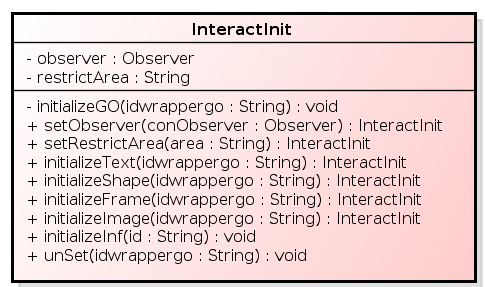
\includegraphics[scale=0.90]{img/diacla/InteractInit.png}
\caption{Diagramma della classe premi/client/editor/lib/InteractInit}
\end{center}
\end{figure}

\begin{description}
%-------  descrizione della classe%
\item[Descrizione] \hfill
	classe che contiene i metodi per la gestione del ridimensionamento e dello spostamento degli oggetti. 
	
	\item[Dipendenze] \hfill
	\begin{itemize}
		\item \textbf{Observer}: per osservare l'oggetto inizializzato con interactjs. In molti metodi vengono usati le funzioni \textit{on(signal,func)} e \textit{emit(signal,param1,param2,param3,param4)} di Observer per emettere dei segnali.
	\end{itemize}
	
%-------  lista degli Attributi%	
\item[Attributi] \hfill
	\begin{description}
		\item[\textbf{- observer : Observer			}] \hfill
			oggetto Observer che viene utilizzato per osservare un oggetto grafico;
		\item[\textbf{- 	restrictArea : String		}] \hfill
			identifica l'area in cui un oggetto può essere spostato.
	\end{description}
	
	
%-------  lista dei metodi%	
\item[Metodi] \hfill

	% -- inizio metodo -- %
	\begin{description}
		\item[\textbf{\color{blue}- initializeGO(idwrapperGO : String	) : void		}] \hfill
			inizializza un oggetto grafico impostando l'area di restrizione e impostando l'observer sull'oggetto. Si appoggia alla libreria interact e sulla classe observer.
			
		\begin{description}
			\item[Argomenti] \hfill
				\begin{itemize}
				
					\item \textbf{idwrapperGO : String			} \hfill
						Identifica l'id dell'oggetto da inizializzare.
					
				\end{itemize}
		\end{description}
	\end{description}		

	\begin{description}
		\item[\textbf{\color{blue}+ setObserver(conObserver : Observer) : interactInit			}] \hfill
			imposta un oggetto Observer sull'oggetto da controllare. restituisce un riferimento dell'oggetto interactInit.
			
		\begin{description}
			\item[Argomenti] \hfill
				\begin{itemize}
				
					\item \textbf{conObserver : Observer			} \hfill
						Identifica l'observer da impostare sull'oggetto.
					
				\end{itemize}
		\end{description}
	\end{description}			

	\begin{description}
		\item[\textbf{\color{blue}+ setRestrictArea(area : String) : interactInit			}] \hfill
			imposta l'area di restrizione entro cui un oggetto può essere spostato. Restituisce un riferimento dell'oggetto interactInit.
			
		\begin{description}
			\item[Argomenti] \hfill
				\begin{itemize}
				
					\item \textbf{area : String			} \hfill
						Identifica l'area di restrizione.
					
				\end{itemize}
		\end{description}
	\end{description}
	
		\begin{description}
		\item[\textbf{\color{blue}+ initializeText(idwrappergo : String) : interactInit			}] \hfill
			inizializza un determinato oggetto di tipo text. Restituisce un riferimento dell'oggetto interactInit.
			
		\begin{description}
			\item[Argomenti] \hfill
				\begin{itemize}
				
					\item \textbf{idwrappergo : String			} \hfill
						Identifica l'id dell'oggetto text da inizializzare.
					
				\end{itemize}
		\end{description}
	\end{description}	
	
\begin{description}
		\item[\textbf{\color{blue}+ initializeShape(idwrappergo : String) : interactInit			}] \hfill
			inizializza un determinato oggetto di tipo shape impostando il comportamento per lo spostamento e ridimensionamento dell'oggetto. Restituisce un riferimento dell'oggetto interactInit.
			
		\begin{description}
			\item[Argomenti] \hfill
				\begin{itemize}
				
					\item \textbf{idwrappergo : String			} \hfill
						Identifica l'id dell'oggetto shape da inizializzare.
					
				\end{itemize}
		\end{description}
	\end{description}	

\begin{description}
		\item[\textbf{\color{blue}+ initializeFrame(idwrappergo : String) : interactInit			}] \hfill
			inizializza un determinato oggetto di tipo frame. Restituisce un riferimento dell'oggetto interactInit.
			
		\begin{description}
			\item[Argomenti] \hfill
				\begin{itemize}
				
					\item \textbf{idwrappergo : String			} \hfill
						Identifica l'id dell'oggetto frame da inizializzare.
					
				\end{itemize}
		\end{description}
	\end{description}
	
\begin{description}
		\item[\textbf{\color{blue}+ initializeImage(idwrappergo : String) : interactInit			}] \hfill
			inizializza un determinato oggetto di tipo image impostando i comportamenti per lo spostamento e il ridimensionamento dell'oggetto. Restituisce un riferimento dell'oggetto interactInit.
			
		\begin{description}
			\item[Argomenti] \hfill
				\begin{itemize}
				
					\item \textbf{idwrappergo : String			} \hfill
						Identifica l'id dell'oggetto image da inizializzare.
					
				\end{itemize}
		\end{description}
	\end{description}
	
\begin{description}
		\item[\textbf{\color{blue}+ initializeInf(id : String) : interactInit			}] \hfill
			inizializza un determinato oggetto di tipo infografica. Restituisce un riferimento dell'oggetto interactInit.
			
		\begin{description}
			\item[Argomenti] \hfill
				\begin{itemize}
				
					\item \textbf{idwrappergo : String			} \hfill
						Identifica l'id dell'oggetto infografica da inizializzare.
					
				\end{itemize}
		\end{description}
	\end{description}

\begin{description}
		\item[\textbf{\color{blue}+ unSet(idwrappergo : String) : interactInit			}] \hfill
			disabilita interactjs per un determinato oggetto togliendo la possibilità di ridimensionamento e spostamento dell'oggetto.
			
		\begin{description}
			\item[Argomenti] \hfill
				\begin{itemize}
				
					\item \textbf{idwrappergo : String			} \hfill
						Identifica l'id dell'oggetto su cui disabilitare interactjs.
					
				\end{itemize}
		\end{description}
	\end{description}
		
	
	
	
\end{description}

%-------  diagramma della classe%
\subsubsection{premi/client/client/lib/Observer}
\begin{figure}[H]
\begin{center}
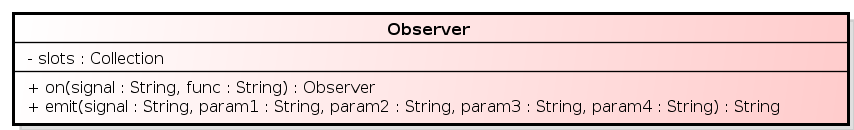
\includegraphics[scale=0.70]{img/diacla/Observer.png}
\caption{Diagramma della classe premi/client/editor/lib/Observer}
\end{center}
\end{figure}

\begin{description}
%-------  descrizione della classe%
\item[Descrizione] \hfill
	è la classe che si occupa di osservare degli oggetti grafici impostando e inviando dei segnali.
		
	
%-------  lista degli Attributi%	
\item[Attributi] \hfill
	\begin{description}
		\item[\textbf{- slots : Collection			}] \hfill
			array di oggetti JSON in cui la chiave rappresenta un segnale e il valore l'azione da intraprendere.
	\end{description}
	
	
%-------  lista dei metodi%	
\item[Metodi] \hfill

	\begin{description}
		\item[\textbf{\color{blue}+ on(signal : String, func : String) : Observer			}] \hfill
			assegna la funzione func al segnale signal. Restituisce un riferimento di Observer.
			
		\begin{description}
			\item[Argomenti] \hfill
				\begin{itemize}
				
					\item \textbf{signal : String			} \hfill
					identifica il nome del segnale;
					\item \textbf{func : String			} \hfill
					identifica la funzione da eseguire al verificarsi del segnale;			
				\end{itemize}
		\end{description}
	\end{description}		
	
	\begin{description}
		\item[\textbf{\color{blue}+ emit(signal : String, param1 : String, param2 : String, param3 : String, param4 : String) : String			}] \hfill
			Restituisce lo slot con un determinato segnale e con determinati parametri.
			
		\begin{description}
			\item[Argomenti] \hfill
				\begin{itemize}
				
					\item \textbf{signal : String			} \hfill
					identifica il nome del segnale;
					\item \textbf{param1,param2,param3,param4 : String			} \hfill
					identificano i parametri del segnale signal;			
				\end{itemize}
		\end{description}
	\end{description}		
	
	
\end{description}

%-------  diagramma della classe%
\subsubsection{premi/client/editor/lib/saver}
\begin{figure}[H]
\begin{center}
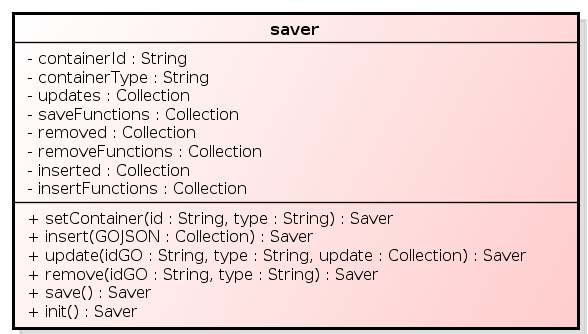
\includegraphics[scale=0.90]{img/diacla/Saver.png}
\caption{Diagramma della classe premi/client/editor/lib/Saver}
\end{center}
\end{figure} 
 
\begin{description}
%-------  descrizione della classe%
\item[Descrizione] \hfill
	rappresenta un oggetto che permette ad un contenitore di oggetti di interfacciarsi con il database ed effettuare le modifiche. L'oggetto saver riceve dal contenitore una serie di operazioni da eseguire sul database e le esegue rispettando i suoi tempi di risposta.
	
	
%-------  lista degli Attributi%	
\item[Attributi] \hfill
	\begin{description}
		\item[\textbf{- containerId : String			}] \hfill
			identifica l'id dell'oggetto da interfacciare con il database;
		\item[\textbf{- containerType : String			}] \hfill
			identifica il tipo dell'oggetto da interfacciare con il database;
		\item[\textbf{- updates : Collection			}] \hfill
			contiene le operazioni di aggiornamento da eseguire nel db. E' un oggetto JSON che contiene i seguenti campi:
			\begin{itemize}
				\item \textit{image:} oggetto JSON che contiene le modifiche sugli oggetti image;
				\item \textit{shape:} oggetto JSON che contiene le modifiche sugli oggetti shape;
				\item \textit{text:} oggetto JSON che contiene le modifiche sugli oggetti text;
				\item \textit{frame:} oggetto JSON che contiene le modifiche sugli oggetti frame;
				\item \textit{infographic:} oggetto JSON che contiene le modifiche sugli oggetti infographic.
			\end{itemize}
			
			Il seguente è l'oggetto JSON inizializzato con i valori di default:
\begin{lstlisting}
{
    "image"               : {},
    "shape"               : {},
    "text"                : {},
    "frame"               : {},
    "infographic"         : {}    
}
\end{lstlisting}					

		\item[\textbf{- saveFunctions : Collection			}] \hfill
			contiene i nomi delle funzioni che si occupano di salvare degli oggetti nel database. I campi che contiene sono:
			\begin{itemize}
				\item \textit{image:} contiene la funzione che si occupa di salvare le image;
				\item \textit{shape:} contiene la funzione che si occupa di salvare gli shape;
				\item \textit{text:} contiene la funzione che si occupa di salvare i text;
				\item \textit{frame:} contiene la funzione che si occupa di salvare i frame;
				\item \textit{infographic:} contiene la funzione che si occupa di salvare le infographic.
			\end{itemize}

Il seguente è l'oggetto JSON inizializzato con i valori di default:
			\begin{lstlisting}
{
    "image"               : databaseAPI.updateSimpleGOContent,
    "shape"               : databaseAPI.updateSimpleGOContent,
    "text"                : databaseAPI.updateSimpleGOContent,
    "frame"               : databaseAPI.updateFrame,
    "infographic"         : databaseAPI.updateInfographic   
}
			\end{lstlisting}				
					
	\item[\textbf{- removed : Collection			}] \hfill
			contiene le operazioni di rimozione da eseguire nel db. E' un oggetto JSON che contiene i seguenti campi:
			\begin{itemize}
				\item \textit{image:} oggetto JSON che contiene le operazioni di rimozione degli oggetti image;
				\item \textit{shape:} oggetto JSON che contiene le operazioni di rimozione degli oggetti shape;
				\item \textit{text:} oggetto JSON che contiene le operazioni di rimozione degli oggetti text;
				\item \textit{frame:} oggetto JSON che contiene le operazioni di rimozione degli oggetti frame;
				\item \textit{infographic:} oggetto JSON che contiene le operazioni di rimozione degli oggetti infographic.
			\end{itemize}
			
			Il seguente è l'oggetto JSON inizializzato con i valori di default:
			\begin{lstlisting}
{
    "image"               : [],
    "shape"               : [],
    "text"                : [],
    "frame"               : [] 
}
			\end{lstlisting}					
	\item[\textbf{- removeFunctions : Collection			}] \hfill
			contiene i nomi delle funzioni che si occupano di rimuovere degli oggetti dal database. I campi che contiene sono:
			\begin{itemize}
				\item \textit{image:} contiene la funzione che si occupa di rimuovere le image;
				\item \textit{shape:} contiene la funzione che si occupa di rimuovere gli shape;
				\item \textit{text:} contiene la funzione che si occupa di rimuovere i text;
				\item \textit{frame:} contiene la funzione che si occupa di rimuovere i frame;
				\item \textit{infographic:} contiene la funzione che si occupa di rimuovere l'infographic.
			\end{itemize}
			
			Il seguente è l'oggetto JSON inizializzato con i valori di default:
			\begin{lstlisting}
{
    "image"               : databaseAPI.removeSimpleGOContent,
    "shape"               : databaseAPI.removeSimpleGOContent,
    "text"                : databaseAPI.removeSimpleGOContent,
    "frame"               : databaseAPI.removeFrameInfographic 
}
			\end{lstlisting}					
	\item[\textbf{- inserted : Collection			}] \hfill
			contiene le operazioni di inserimento da eseguire nel db. E' un oggetto JSON che contiene i seguenti campi:
			\begin{itemize}
				\item \textit{image:} oggetto JSON che contiene le operazioni di inserimento degli oggetti image;
				\item \textit{shape:} oggetto JSON che contiene le operazioni di inserimento degli oggetti shape;
				\item \textit{text:} oggetto JSON che contiene le operazioni di inserimento degli oggetti text;
				\item \textit{frame:} oggetto JSON che contiene le operazioni di inserimento degli oggetti frame;
				\item \textit{infographic:} oggetto JSON che contiene le operazioni di inserimento degli oggetti infographic.
			\end{itemize}
			
			Il seguente è l'oggetto JSON inizializzato con i valori di default:
			\begin{lstlisting}
{
    "image"               : [],
    "shape"               : [],
    "text"                : [],
    "frame"               : [] 
}
			\end{lstlisting}	
			\item[\textbf{- insertFunctions : Collection			}] \hfill
			contiene i nomi delle funzioni che si occupano di inserire degli oggetti sul database. I campi che contiene sono:
			\begin{itemize}
				\item \textit{image:} contiene la funzione che si occupa di inserire le image;
				\item \textit{shape:} contiene la funzione che si occupa di inserire gli shape;
				\item \textit{text:} contiene la funzione che si occupa di inserire i text;
				\item \textit{frame:} contiene la funzione che si occupa di inserire i frame;
				\item \textit{infographic:} contiene la funzione che si occupa di inserire l'infographic.
			\end{itemize}

Il seguente è l'oggetto JSON inizializzato con i valori di default:
			\begin{lstlisting}
{
    "image"               : databaseAPI.insertSimpleGOContent,
    "shape"               : databaseAPI.insertSimpleGOContent,
    "text"                : databaseAPI.insertSimpleGOContent,
    "frame"               : databaseAPI.insertFrameInfographic 
}
			\end{lstlisting}								
		
	\end{description}
	
	
%-------  lista dei metodi%	
\item[Metodi] \hfill

	% -- inizio metodo -- %
	\begin{description}
		\item[\textbf{\color{blue}+ setContainer(id : String, type : String) : Saver			}] \hfill
			imposta il container da interfacciare con il Saver. Restituisce un riferimento dell'oggetto Saver.
			
		\begin{description}
			% -- lista argomenti del metodo -- %
			\item[Argomenti] \hfill
				\begin{itemize}
				
					\item \textbf{id : String			} \hfill
					identificativo del container;
					\item \textbf{type : String			} \hfill
					definisce il tipo del container.
				\end{itemize}
		\end{description}
	\end{description}	

	\begin{description}
		\item[\textbf{\color{blue}+ insert(GOJSON : Collection) : Saver			}] \hfill
			inserisce un operazione di inserimento da eseguire nel campo inserted. Restituisce un riferimento dell'oggetto Saver.
			
		\begin{description}
			% -- lista argomenti del metodo -- %
			\item[Argomenti] \hfill
				\begin{itemize}
				
					\item \textbf{GOJSON : Collection			} \hfill
					oggetto JSON che dev'essere inserito nel database.
				\end{itemize}
		\end{description}
	\end{description}	

	\begin{description}
		\item[\textbf{\color{blue}+ update(idGO : String, type : String, update : Collection) : Saver			}] \hfill
			inserisce un operazione di modifica, nel campo updates. Restituisce un riferimento dell'oggetto Saver.
			
		\begin{description}
			% -- lista argomenti del metodo -- %
			\item[Argomenti] \hfill
				\begin{itemize}
				
					\item \textbf{idGO : String			} \hfill
					identifica l'id dell'oggetto da modificare;
					\item \textbf{type : String			} \hfill
					identifica il tipo dell'oggetto da modificare;
					\item \textbf{update : Collection			} \hfill
					oggetto JSON che contiene le modifiche da apportare sul db. 
				\end{itemize}
		\end{description}
	\end{description}

	\begin{description}
		\item[\textbf{\color{blue}+ remove(idGO : String, type : String) : Saver			}] \hfill
			inserisce un operazione di rimozione di un oggetto, nel campo removed. Restituisce un riferimento dell'oggetto Saver.
			
		\begin{description}
			% -- lista argomenti del metodo -- %
			\item[Argomenti] \hfill
				\begin{itemize}
				
					\item \textbf{idGO : String			} \hfill
					identifica l'id dell'oggetto da rimuovere;
					\item \textbf{type : String			} \hfill
					identifica il tipo dell'oggetto da rimuovere;
				\end{itemize}
		\end{description}
	\end{description}
	
		\begin{description}
		\item[\textbf{\color{blue}+ save() : Saver			}] \hfill
			esegue le operazioni pendenti di inserimento, modifica e rimozione sul database. Restituisce un riferimento dell'oggetto Saver.
		\end{description}

		\begin{description}
		\item[\textbf{\color{blue}+ init() : Saver			}] \hfill
			inizializza i campi dell'oggetto Saver. Restituisce un riferimento dell'oggetto Saver.
		\end{description}	
	
\end{description}


\subsubsection{premi/client/editor/lib/Shape}
\begin{figure}[H]
\begin{center}
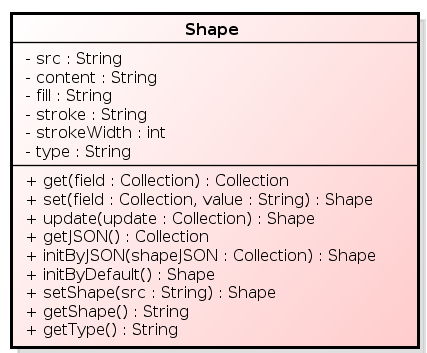
\includegraphics[scale=0.80]{img/diacla/shape.png}
\caption{Diagramma della classe premi/client/editor/lib/Shape}
\end{center}
\end{figure}

\begin{description}
%-------  descrizione della classe%
\item[Descrizione] \hfill
	è una classe che rappresenta un oggetto shape. Contiene i metodi per gestire uno shape.
	
\item[Classi ereditate] \hfill
	\begin{itemize}
		\item GObject
	\end{itemize}
	
%-------  lista degli Attributi%	
\item[Attributi] \hfill
	\begin{description}
		\item[\textbf{- info : Collection			}] \hfill
			l'attributo info è un oggetto JSON che estende l'attributo info ereditato da GObject. I campi aggiuntivi sono:
	\begin{itemize}
		\item \textit{src:} definisce il percorso dello shape da visualizzare. Ogni shape è rappresentato da un immagine svg;
		\item \textit{content:} definisce il contenuto dello shape;		
		\item \textit{fill:} definisce il colore della parte interna dell'oggetto grafico; %da chiarire
        \item \textit{stroke:} definisce il colore del bordo dell'oggetto grafico; %da chiarire
        \item \textit{strokeWidth:} definisce la dimensione del bordo dell'oggetto grafico; %da chiarire
		\item \textit{type:} identifica il tipo di oggetto.		
	\end{itemize}
	Viene inizializzato dal metodo initByDefault e il seguente è l'oggetto JSON inizializzato con i valori di default:
\begin{lstlisting}
{
    "_id"               : "",    
    "dataX"             : 0,
    "dataY"             : 0,
    "dataZ"             : 0,
    "height"            : 100,
    "width"             : 100,
    "scale"             : 1,
    "lvl"               : 0,
    "src                : "",
    "content"           : "",
    "color"             : "black",
    "stroke"            : "black",
    "strokeWidth"       : 2,
    "path"              : "",
    "y"                 : "",
    "viewBox"           : "",
    "style"             : "",
    "zoom"              : 100,
    "sWidth"            : 0,
    "sHeight"           : 0,
    "type"              : 'shape'
}
\end{lstlisting}					
                 L'attributo Info è usato in molti metodi di questa classe. Ad ogni metodo che si interfaccia con questo oggetto, verrà specificato nella descrizione le modifiche che vengono apportate. 	
	\end{description}
	
%-------  lista dei metodi
\item[Metodi] \hfill

\begin{description}
		\item[\textbf{\color{blue}+ get(field : String) : String			}] \hfill
			restituisce una proprietà dell'oggetto shape.
			
		\begin{description}
			% -- lista argomenti del metodo -- %
			\item[Argomenti] \hfill
				\begin{itemize}
				
					\item \textbf{field : String			} \hfill
					identifica la proprietà da restituire;
				\end{itemize}
		\end{description}

\end{description}


		\begin{description}
		\item[\textbf{\color{blue}+ set(field : String, value : String) : Shape			}] \hfill
			permette di settare un campo dell'attributo info. Restituisce un riferimento dell'oggetto Shape.
			
		\begin{description}
			% -- lista argomenti del metodo -- %
			\item[Argomenti] \hfill
				\begin{itemize}
				
					\item \textbf{field : String			} \hfill
					identifica il campo da settare di info;
					\item \textbf{value : String			} \hfill
					rappresenta il valore del campo da settare su l'attributo info.
				\end{itemize}
		\end{description}

\end{description}

\begin{description}
		\item[\textbf{\color{blue}+ update(update : Collection) : Shape			}] \hfill
			permette di aggiornare i campi dell'attributo info. Restituisce un riferimento dell'oggetto Shape.
			
		\begin{description}
			% -- lista argomenti del metodo -- %
			\item[Argomenti] \hfill
				\begin{itemize}
				
					\item \textbf{update : Collection			} \hfill
					update è un oggetto JSON che contiene chiave e valore dei campi che devono essere aggiornati. 
				\end{itemize}
		\end{description}

\end{description}

\begin{description}
		\item[\textbf{\color{blue}+ initByJSON(shapeJSON : Collection) : Shape			}] \hfill
			permette di inizializzare l'attributo info tramite un oggetto JSON.  
			Restituisce un riferimento dell'oggetto Shape.
		\begin{description}
			% -- lista argomenti del metodo -- %
			\item[Argomenti] \hfill
				\begin{itemize}
				
					\item \textbf{shapeJSON : Collection			} \hfill
					è un oggetto JSON che contiene chiave e valore di inizializzazione dei campi dell'attributo info. 
				\end{itemize}
		\end{description}

\end{description}

\begin{description}
		\item[\textbf{\color{blue}+ initByDefault() : Shape			}] \hfill
			permette di inizializzare i campi dell'attributo info con i parametri di default. Restituisce un riferimento dell'oggetto Shape. 

\end{description}

\begin{description}
		\item[\textbf{\color{blue}+ setShape(src : String) : Shape			}] \hfill
			setta l'url(percorso) dello shape. Restituisce un riferimento dell'oggetto Shape.
			
		\begin{description}
			% -- lista argomenti del metodo -- %
			\item[Argomenti] \hfill
				\begin{itemize}
				
					\item \textbf{src : String			} \hfill
					identifica l'url(percorso) dello shape.
				\end{itemize}
		\end{description}

\end{description}

\begin{description}
		\item[\textbf{\color{blue}+ getShape() : String			}] \hfill
			restituisce l'url(percorso) dello shape. 

\end{description}

\begin{description}
		\item[\textbf{\color{blue}+ getType() : String			}] \hfill
			restituisce la stringa "shape" per identificare che il tipo dell'oggetto è image. 

\end{description}



\end{description}


\subsubsection{premi/client/editor/lib/Text}
\begin{figure}[H]
\begin{center}
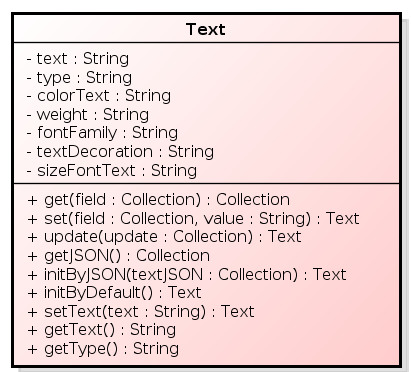
\includegraphics[scale=0.80]{img/diacla/text.png}
\caption{Diagramma della classe premi/client/editor/lib/Text}
\end{center}
\end{figure}

\begin{description}
%-------  descrizione della classe%
\item[Descrizione] \hfill
	è una classe che rappresenta un oggetto text. Contiene i metodi per gestire uno text.
	
\item[Classi ereditate] \hfill
	\begin{itemize}
		\item GObject
	\end{itemize}
	
%-------  lista degli Attributi%	
\item[Attributi] \hfill
	\begin{description}
		\item[\textbf{- info : Collection			}] \hfill
			l'attributo info è un oggetto JSON che estende l'attributo info ereditato da GObject. I campi aggiuntivi sono:
	\begin{itemize}
		\item \textit{text:} definisce il testo da visualizzare sull'oggetto;
		\item \textit{colorText:} definisce il colore del testo;		
		\item \textit{weight:} definisce la larghezza del testo;
        \item \textit{fontFamily:} definisce il font del testo;
        \item \textit{textDecoration:} definisce particolari decorazioni da attribuire al testo; 
        \item \textit{sizeFontText:} definisce la grandezza del testo;
		\item \textit{type:} identifica il tipo di oggetto.		
	\end{itemize}
	Viene inizializzato dal metodo initByDefault e il seguente è l'oggetto JSON inizializzato con i valori di default:
\begin{lstlisting}
{
    "_id"               : "",    
    "dataX"             : 0,
    "dataY"             : 0,
    "dataZ"             : 0,
    "height"            : 100,
    "width"             : 100,
    "scale"             : 1,
    "lvl"               : 0,
    "text"              : "text",
    "type"              : 'text',
    "color"             : '#ffffff',
    "weight"            : '',
    "fontStyle"         : '',
    "textDecoration"    : '',
    "sizeFontText"      : '20',
    "fontFamily"        : 'Arial'
}
\end{lstlisting}					
                 L'attributo Info è usato in molti metodi di questa classe. Ad ogni metodo che si interfaccia con questo oggetto, verrà specificato nella descrizione le modifiche che vengono apportate.
	\end{description}
	
%-------  lista dei metodi
\item[Metodi] \hfill

\begin{description}
		\item[\textbf{\color{blue}+ get(field : String) : String			}] \hfill
			restituisce una proprietà dell'oggetto text.
			
		\begin{description}
			% -- lista argomenti del metodo -- %
			\item[Argomenti] \hfill
				\begin{itemize}
				
					\item \textbf{field : String			} \hfill
					identifica la proprietà da restituire;
				\end{itemize}
		\end{description}

\end{description}


		\begin{description}
		\item[\textbf{\color{blue}+ set(field : String, value : String) : Text			}] \hfill
			permette di settare un campo dell'attributo info. Restituisce un riferimento dell'oggetto Text.
			
		\begin{description}
			% -- lista argomenti del metodo -- %
			\item[Argomenti] \hfill
				\begin{itemize}
				
					\item \textbf{field : String			} \hfill
					identifica il campo da settare di info;
					\item \textbf{value : String			} \hfill
					rappresenta il valore del campo da settare su l'attributo info.
				\end{itemize}
		\end{description}

\end{description}

\begin{description}
		\item[\textbf{\color{blue}+ update(update : Collection) : Text			}] \hfill
			permette di aggiornare i campi dell'attributo info. Restituisce un riferimento dell'oggetto Text.
			
		\begin{description}
			% -- lista argomenti del metodo -- %
			\item[Argomenti] \hfill
				\begin{itemize}
				
					\item \textbf{update : Collection			} \hfill
					update è un oggetto JSON che contiene chiave e valore dei campi che devono essere aggiornati. 
				\end{itemize}
		\end{description}

\end{description}

\begin{description}
		\item[\textbf{\color{blue}+ initByJSON(textJSON : Collection) : Text			}] \hfill
			permette di inizializzare l'attributo info tramite un oggetto JSON. Restituisce un riferimento dell'oggetto Text. 
			
		\begin{description}
			% -- lista argomenti del metodo -- %
			\item[Argomenti] \hfill
				\begin{itemize}
				
					\item \textbf{textJSON : Collection			} \hfill
					è un oggetto JSON che contiene chiave e valore di inizializzazione dei campi dell'attributo info. 
				\end{itemize}
		\end{description}

\end{description}

\begin{description}
		\item[\textbf{\color{blue}+ initByDefault() : Text			}] \hfill
			permette di inizializzare i campi dell'attributo info con i parametri di default. Restituisce un riferimento dell'oggetto Text. 

\end{description}

\begin{description}
		\item[\textbf{\color{blue}+ setText(text : String) : Collection			}] \hfill
			setta il testo del text.
			
		\begin{description}
			% -- lista argomenti del metodo -- %
			\item[Argomenti] \hfill
				\begin{itemize}
				
					\item \textbf{text : String			} \hfill
					identifica il testo da inserire.
				\end{itemize}
		\end{description}

\end{description}

\begin{description}
		\item[\textbf{\color{blue}+ getText() : String			}] \hfill
			restituisce il testo dell'oggetto. 

\end{description}

\begin{description}
		\item[\textbf{\color{blue}+ getType() : String			}] \hfill
			restituisce la stringa "shape" per identificare che il tipo dell'oggetto è image. 

\end{description}



\end{description}










